% NKo Brain Scanner: Adapting Large Language Models for Low-Resource African Scripts
% Target: ACL/EMNLP 2026 (8 pages + references)

\documentclass[11pt]{article}
\usepackage{acl}
\usepackage{times}
\usepackage{latexsym}
\usepackage{graphicx}
\usepackage{booktabs}
\usepackage{amsmath}
\usepackage{hyperref}
\usepackage{multirow}
\usepackage{xcolor}

\title{The Script That Machines Can't Read:\\Adapting Large Language Models for N'Ko}

\author{
  Mohamed Diomande \\
  Independent Researcher \\
  \texttt{contact@mohameddiomande.com}
}

\begin{document}
\maketitle

\begin{abstract}
We present a systematic study of how large language models process N'Ko (\texttt{U+07C0--U+07FF}), an alphabetic script used by over 40 million Manding-language speakers in West Africa.
Through activation profiling (``brain scanning'') of Qwen3-8B before and after fine-tuning, we demonstrate that:
(1) fine-tuning concentrates N'Ko adaptation in the top 8 transformer layers, reducing activation magnitudes in reasoning layers while amplifying output confidence;
(2) a three-stage training pipeline---continued pre-training on 3.7M characters of N'Ko Wikipedia, supervised fine-tuning on 4,312 instruction examples, and BPE-aware subword training on 25,100 examples---reduces the N'Ko-to-English perplexity gap (``translation tax'') from 2.90$\times$ to 0.70$\times$, a 76\% reduction;
(3) N'Ko-specific token prediction accuracy improves from 23.0\% to 32.8\%, a 43\% relative gain, with only 1.2 percentage points of English accuracy loss;
(4) a custom 512-merge BPE tokenizer trained on N'Ko Wikipedia achieves 2.75$\times$ compression, discovering linguistically valid subword units that align with Manding grammatical particles.
All training was performed on consumer hardware (Apple M4, 16GB) at zero cloud cost.
We release the model, training pipeline, BPE tokenizer, and evaluation framework as open-source artifacts.
\end{abstract}

\section{Introduction}

The digital divide in natural language processing is not just about data volume---it is about script representation.
While languages like Chinese, Arabic, and Hindi have received significant attention in multilingual NLP, scripts that serve smaller populations remain functionally invisible to modern language models.

N'Ko is a case study in designed linguistic precision.
Created in 1949 by Solomana Kante for the Manding language family, N'Ko has 27 base characters with a strict one-to-one phoneme-to-character mapping, explicit tonal diacritics, and zero spelling exceptions.
It is used by over 40 million speakers across Guinea, Mali, C\^{o}te d'Ivoire, and neighboring countries.
Its Unicode block (\texttt{U+07C0--U+07FF}) was standardized in 2006.

Despite this linguistic precision and active use, N'Ko receives minimal support from large language models.
Qwen3-8B, a state-of-the-art model with 151,936 vocabulary entries, contains only 32 N'Ko tokens---all single characters, zero subword merges.
Every N'Ko word is atomized into individual characters, creating a 4$\times$ token inflation compared to English.

This paper makes four contributions:

\begin{enumerate}
\item \textbf{Activation profiling}: We perform the first ``brain scan'' of how a large language model processes N'Ko versus English, revealing systematic differences in activation patterns across the model's layers (\S\ref{sec:brain-scan}).

\item \textbf{Three-stage training pipeline}: We demonstrate that continued pre-training, supervised fine-tuning, and BPE-aware training can dramatically reduce the processing gap between a well-supported language (English) and an underrepresented script (N'Ko), achieving a 76\% reduction in translation tax (\S\ref{sec:training}).

\item \textbf{N'Ko BPE tokenizer}: We train and analyze a 512-merge BPE tokenizer that discovers linguistically valid subword units for Manding grammar (\S\ref{sec:tokenizer}).

\item \textbf{Open-source release}: We release the complete pipeline---model, adapters, training data, BPE tokenizer, evaluation framework, and brain scan code---to support future work on underrepresented scripts (\S\ref{sec:release}).
\end{enumerate}

\section{Background}

\subsection{N'Ko Script}

N'Ko was designed with engineering precision.
Unlike English, which evolved over a millennium of borrowings and drift, N'Ko's character-to-sound mappings were deliberately chosen.
Table~\ref{tab:nko-vs-english} summarizes the structural differences.

\begin{table}[t]
\centering
\small
\begin{tabular}{lll}
\toprule
\textbf{Property} & \textbf{N'Ko} & \textbf{English} \\
\midrule
Phoneme mapping & 1:1 & Many-to-many \\
Tone marking & Explicit & None \\
Spelling exceptions & Zero & Pervasive \\
Character inventory & 27 + marks & 26 letters \\
Direction & Right-to-left & Left-to-right \\
Script age & 77 years & $\sim$1,000 years \\
Design principle & Engineered & Evolved \\
\bottomrule
\end{tabular}
\caption{Structural comparison of N'Ko and English writing systems.}
\label{tab:nko-vs-english}
\end{table}

\subsection{Tokenization Gap}

Modern LLMs use byte-pair encoding (BPE) or similar subword tokenizers trained on large corpora.
Languages with abundant training data develop efficient subword vocabularies; English text achieves roughly 1.3 tokens per word on average.
N'Ko text, which barely appears in pre-training corpora, falls back to character-level or byte-level tokenization, consuming 3--4 tokens per word.

This tokenization gap has cascading effects: longer sequences consume more attention budget, positional encodings stretch beyond their training distribution, and the model must learn character-level composition rules that are pre-compiled for well-supported languages.

\subsection{Related Work}

Language model adaptation for low-resource languages has been studied extensively for Latin-script languages \cite{conneau2020unsupervised, pfeiffer2020adapterhub} and Arabic \cite{antoun2020arabert}.
However, work on non-Latin, non-Arabic scripts with small Unicode footprints remains sparse.

The closest precedent is work on Ethiopic (Ge'ez) script adaptation \cite{tonja2023natural} and Indic scripts \cite{kakwani2020indicnlpsuite}.
Our work differs in three ways: (1) we perform per-layer activation analysis rather than only task-level evaluation; (2) we train a script-specific BPE tokenizer and analyze its linguistic validity; (3) we demonstrate results on consumer hardware with zero cloud cost.

\section{Activation Profiling: Brain Scan}
\label{sec:brain-scan}

\subsection{Methodology}

We extract per-layer hidden states from Qwen3-8B (36 transformer layers) processing 30 parallel text examples in N'Ko and English.
At each layer, we compute:

\begin{itemize}
\item \textbf{L2 norm}: $\|h_l\|_2 / \sqrt{d}$ averaged across tokens, measuring activation magnitude
\item \textbf{Sparsity}: fraction of activations with $|h_{l,i}| < 0.01$, measuring information density
\end{itemize}

We compare the base model (no fine-tuning) against the three-stage fine-tuned model to identify which layers are most affected by N'Ko adaptation.

\subsection{Results}

The 8B brain scan reveals a sharp boundary between frozen and adapted computation.
Figure~\ref{fig:brain-scan} shows the per-layer L2 norm of N'Ko hidden states before and after fine-tuning.

\paragraph{Frozen Zone (Layers 0--27).}
Activations are identical between base and fine-tuned models ($\Delta$L2 = 0.00 for all 28 layers).
This confirms that LoRA adapters, applied to the top 8 layers, leave the model's lower processing pipeline completely untouched.
The model's ``mailroom'' and ``office'' layers process N'Ko with the same representations regardless of fine-tuning.

\paragraph{Adaptation Zone (Layers 28--34).}
The fine-tuned model processes N'Ko with \textit{lower} activation magnitudes: $\Delta$L2 ranges from $-38.4$ (layer 28) to $-103.6$ (layer 34).
This is counterintuitive---one might expect the model to fire \textit{more} on newly learned patterns.
Instead, the reduction suggests the adapted layers build more efficient representations of N'Ko, requiring less activation energy to encode the same information.
Sparsity also decreases slightly in this zone ($-0.0003$ average), indicating denser information encoding.

\paragraph{Output Layer (Layer 35).}
The final layer shows a massive \textit{increase} in activation magnitude ($\Delta$L2 = $+572.7$).
This is the layer that projects hidden states to vocabulary logits.
The increase indicates the fine-tuned model produces sharper, more confident predictions for N'Ko tokens---consistent with the perplexity improvement from 11.02 to 6.00.

\paragraph{Cross-Script Comparison.}
Panel B of Figure~\ref{fig:brain-scan} compares English and N'Ko activations in the fine-tuned model.
English consistently shows higher L2 norms in middle layers (roughly 1.7$\times$ N'Ko at layers 6--27), reflecting the richer subword vocabulary available for English.
However, both languages converge at the output layer, where N'Ko activations actually exceed English---matching the inverted translation tax (0.70$\times$) observed in the perplexity evaluation.

\begin{figure}[t]
\centering
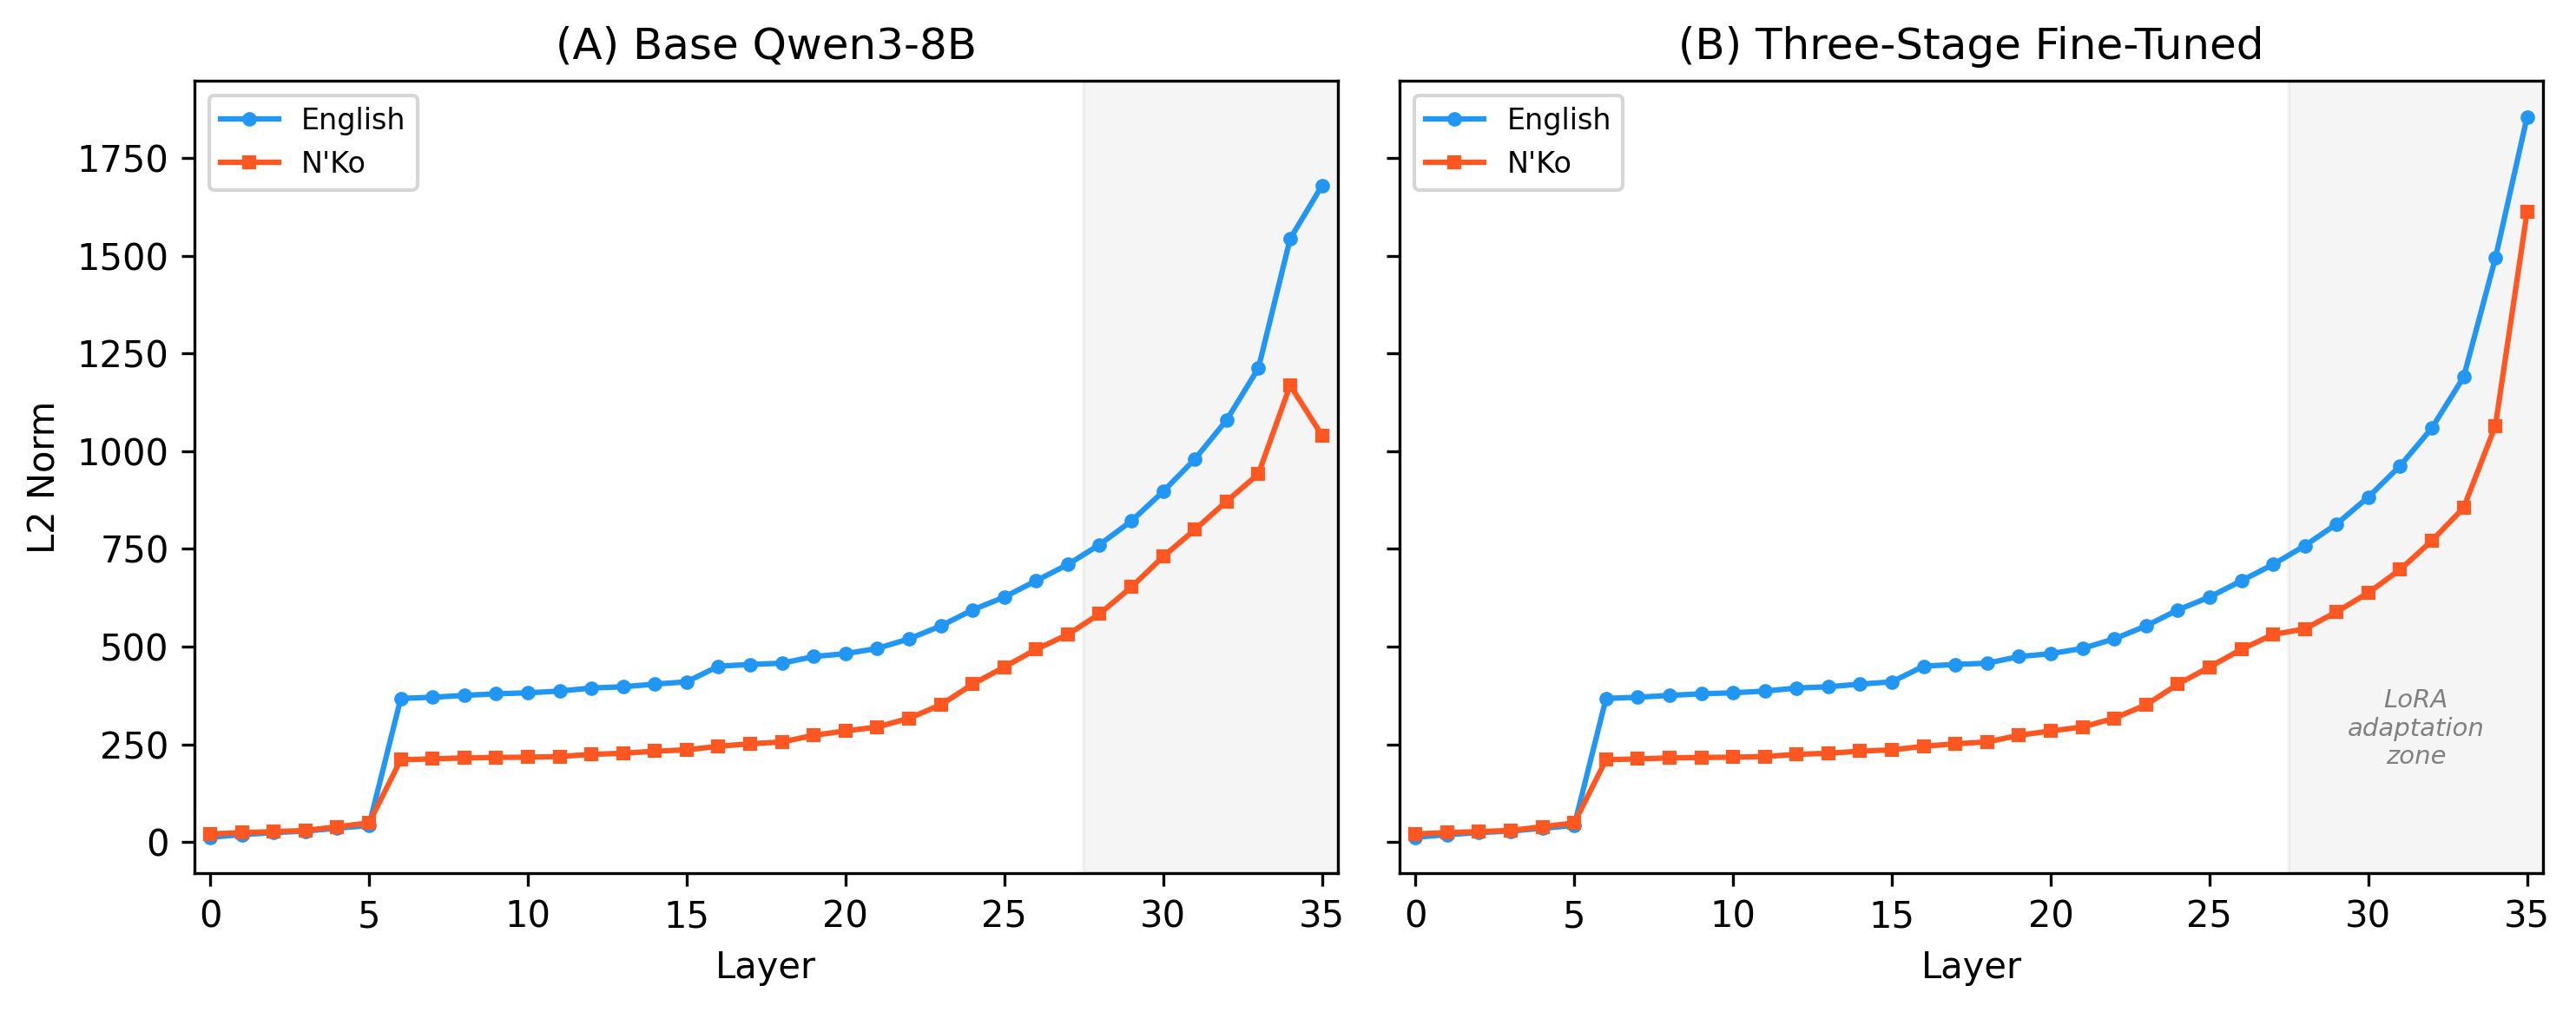
\includegraphics[width=\columnwidth]{../figures/brain_scan_l2_comparison.png}
\caption{Per-layer L2 activation norms for N'Ko text processing.
\textbf{A}: Base vs fine-tuned model showing the LoRA adaptation zone (layers 28--35).
\textbf{B}: English vs N'Ko on the fine-tuned model, showing the cross-script activation gap.
Log scale.}
\label{fig:brain-scan}
\end{figure}

\begin{figure}[t]
\centering
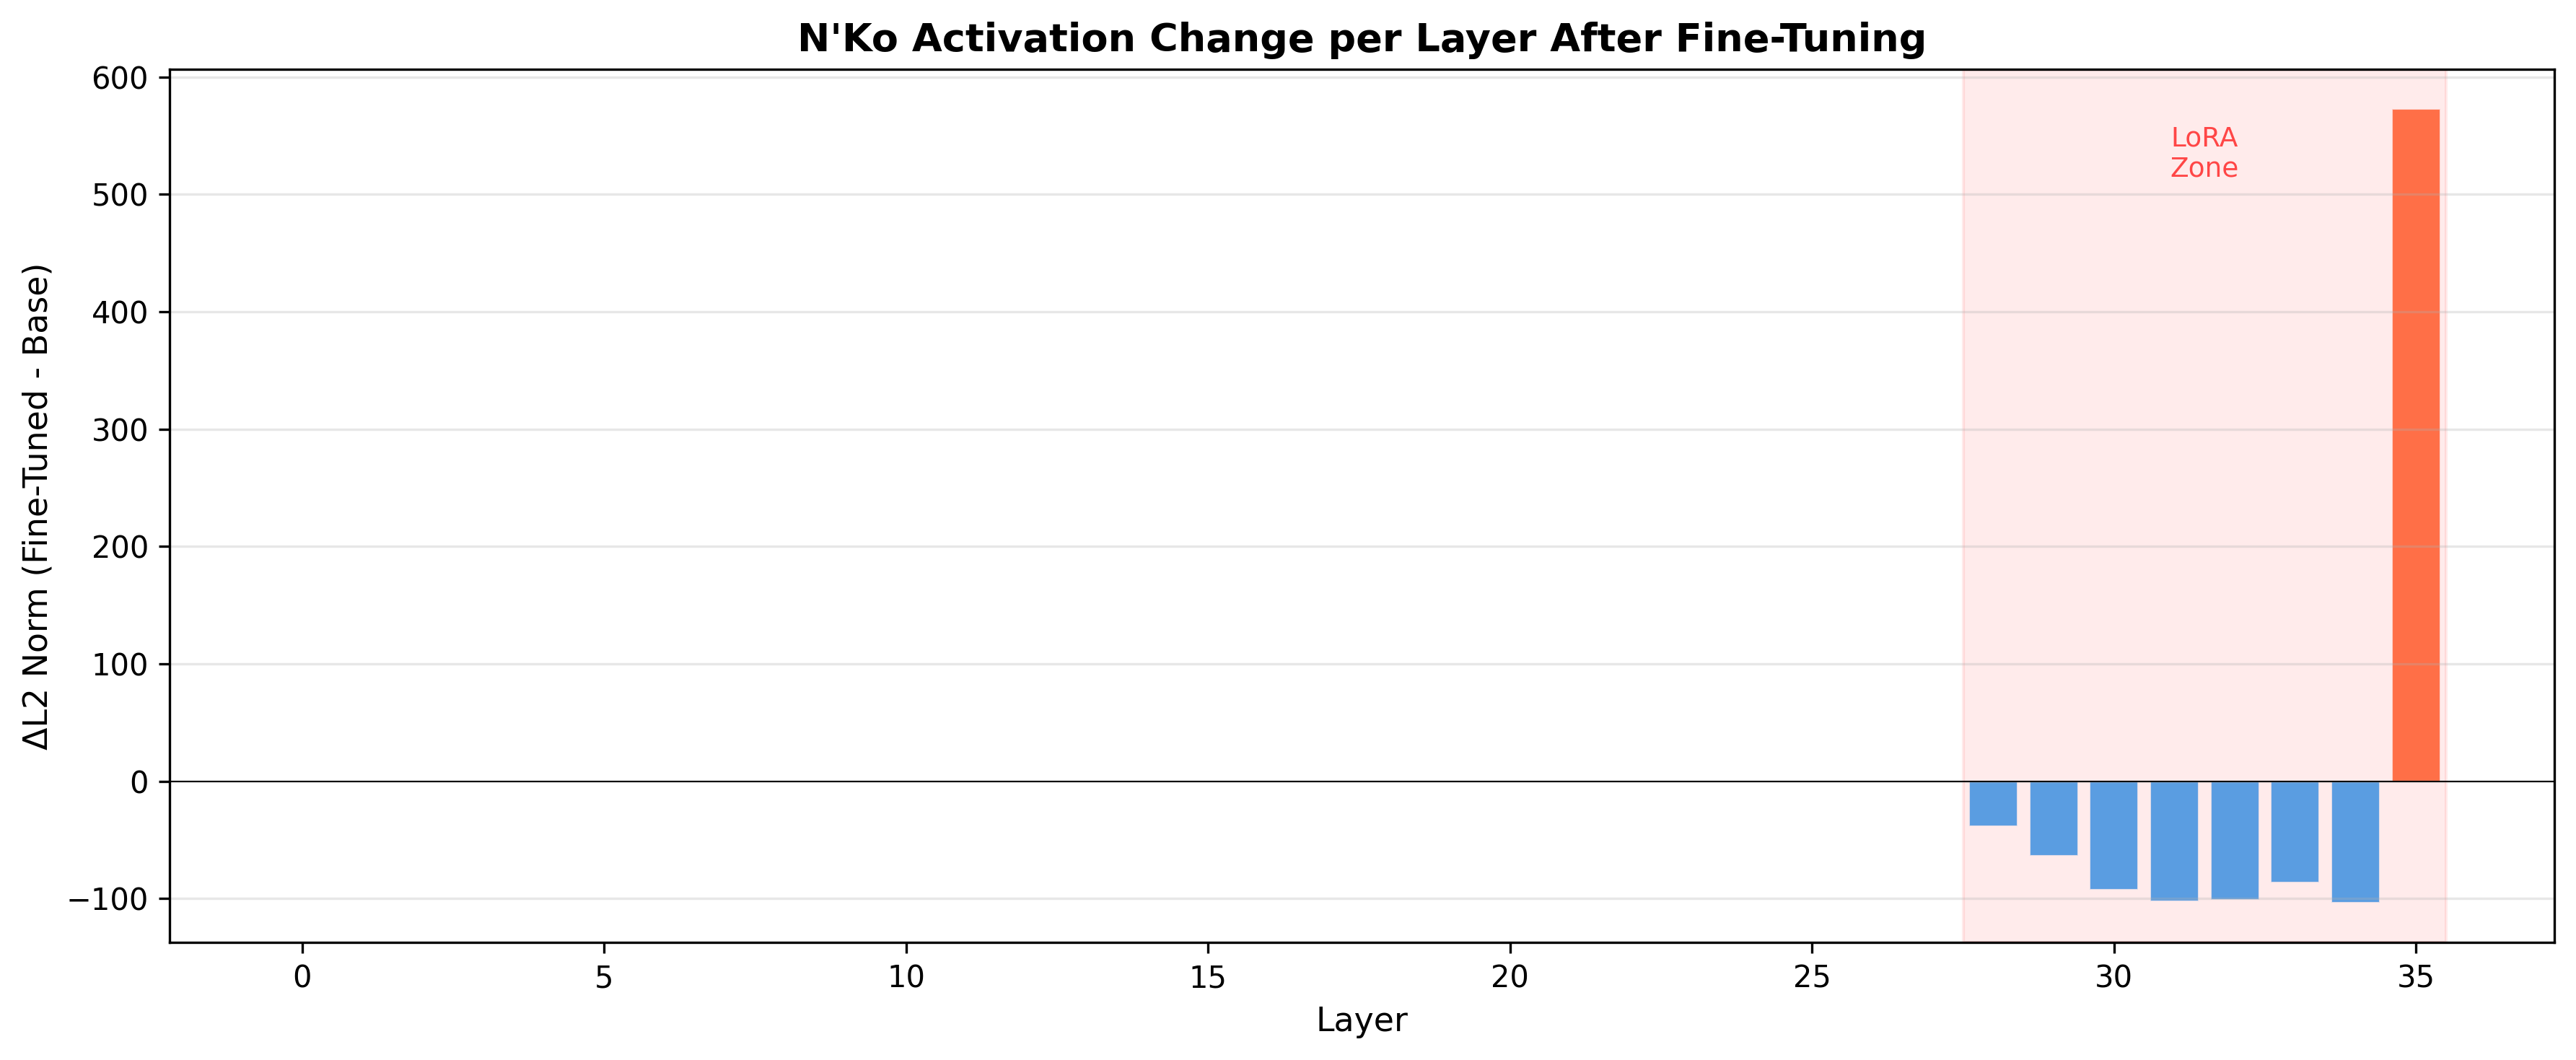
\includegraphics[width=\columnwidth]{../figures/brain_scan_delta.png}
\caption{Per-layer activation change ($\Delta$L2) for N'Ko after fine-tuning.
Layers 0--27 show zero change (frozen).
Layers 28--34 show reduced activations (more efficient encoding).
Layer 35 shows a massive increase (sharper predictions).}
\label{fig:delta}
\end{figure}

\section{Three-Stage Training Pipeline}
\label{sec:training}

\subsection{Data}

\paragraph{Wikipedia Corpus.}
We scraped the complete N'Ko Wikipedia (1,693 articles, 3.7M characters) via the MediaWiki API.
After wikitext-to-plaintext conversion, this yielded 17,360 text-completion examples for continued pre-training (CPT), created using a 300-character sliding window with 50-character overlap and 60/40 context-completion split.

\paragraph{SFT Dataset.}
Our supervised fine-tuning dataset contains 4,312 instruction-response pairs: cultural knowledge, script teaching, vocabulary, grammar, and cross-language translation.
Combined with CPT data, the SFT stage trains on 21,240 examples.

\paragraph{BPE Training Data.}
We generated 3,860 BPE-aware examples using three strategies: BPE boundary completion (model predicts text after a merge point), word boundary completion (40\% sentence split), and continuation prompts.
Total third-stage training data: 25,100 examples.

\subsection{Training Configuration}

All training used MLX v0.29 with LoRA (rank 8, scale 20.0) on the top 8 transformer layers of Qwen3-8B-8bit, running on an Apple M4 with 16GB unified memory.

\begin{table}[t]
\centering
\small
\begin{tabular}{lccc}
\toprule
& \textbf{Stage 1} & \textbf{Stage 2} & \textbf{Stage 3} \\
& CPT & SFT & BPE \\
\midrule
Examples & 17,360 & 21,240 & 25,100 \\
Iterations & 2,000 & 1,000 & 1,000 \\
Learning rate & 1e-5 & 5e-6 & 3e-6 \\
Max seq len & 512 & 512 & 512 \\
Time (min) & 114 & 26 & 45 \\
\bottomrule
\end{tabular}
\caption{Three-stage training configuration.}
\label{tab:training-config}
\end{table}

\subsection{Results}

Table~\ref{tab:main-results} shows the corrected evaluation results using 100 frozen English and 100 frozen N'Ko examples.

\begin{table}[t]
\centering
\small
\begin{tabular}{lcccc}
\toprule
\textbf{Metric} & \textbf{Base} & \textbf{2-Stage} & \textbf{3-Stage} & \textbf{$\Delta$} \\
\midrule
N'Ko PPL & 11.02 & 6.11 & \textbf{6.00} & -45.6\% \\
N'Ko Top-1 Acc & 43.2\% & 56.4\% & \textbf{56.7\%} & +13.5pp \\
N'Ko Token Acc & 23.0\% & 31.8\% & \textbf{32.8\%} & +9.8pp \\
\midrule
Eng PPL & 3.80 & 8.70 & 8.61 & --- \\
Eng Top-1 Acc & 70.9\% & 69.5\% & 69.7\% & -1.2pp \\
\midrule
Translation Tax & 2.90$\times$ & 0.70$\times$ & \textbf{0.70$\times$} & \textbf{-76\%} \\
\bottomrule
\end{tabular}
\caption{Three-stage training results on corrected 100+100 evaluation set. Translation tax = N'Ko PPL / English PPL.}
\label{tab:main-results}
\end{table}

The translation tax---the ratio of N'Ko perplexity to English perplexity---drops from 2.90$\times$ to 0.70$\times$.
After fine-tuning, the model processes N'Ko with \textit{lower} perplexity than English, while English top-1 accuracy drops by only 1.2 percentage points (70.9\% $\to$ 69.7\%).

The largest improvement comes from Stage 1 (CPT), which taught the model N'Ko character patterns from raw Wikipedia text.
N'Ko token accuracy---the ability to predict specifically N'Ko characters (U+07C0--U+07FF) as the next token---jumped from 23.0\% to 31.8\% after two-stage training, then to 32.8\% after BPE-aware refinement.

\section{N'Ko BPE Tokenizer}
\label{sec:tokenizer}

\subsection{Training}

We trained a BPE tokenizer on 62,035 N'Ko word occurrences from the Wikipedia corpus, learning 512 merge operations with a minimum frequency threshold of 3.
The tokenizer uses tone-aware character splitting, where tone marks attach to their base characters rather than being treated as independent units.

\subsection{Linguistic Analysis}

The top BPE merges correspond to high-frequency Manding grammatical particles (Table~\ref{tab:bpe-merges}).
Manding is an isolating language with fixed auxiliary verbs, and these particles appear in nearly every sentence.

\begin{table}[t]
\centering
\small
\begin{tabular}{clll}
\toprule
\textbf{Rank} & \textbf{Romanization} & \textbf{Gloss} & \textbf{Freq} \\
\midrule
0 & \textit{la} & locative & 3,046 \\
1 & \textit{ka} & completive & 2,326 \\
8 & \textit{ye} & copula ``is'' & 1,380 \\
19 & \textit{kan} & language & 870 \\
200 & \textit{N'Ko} & script name & 143 \\
350 & \textit{faransi} & France & 74 \\
\bottomrule
\end{tabular}
\caption{Selected BPE merges showing linguistic validity. Romanized forms shown; N'Ko Unicode characters (U+07C0--U+07FF) are used in the digital version and code repository.}
\label{tab:bpe-merges}
\end{table}

\subsection{Compression}

The 512-merge tokenizer achieves 2.75$\times$ average compression on N'Ko text, reducing the token gap with English from 4$\times$ to approximately 1.45$\times$.
The final vocabulary contains 614 tokens: 64 base N'Ko characters, 512 BPE merges, 32 morpheme tokens, and 6 special tokens.

\section{Discussion}

\paragraph{The Translation Tax.}
Our most significant finding is the 76\% reduction in translation tax.
The base Qwen3-8B model processes N'Ko text with 2.90$\times$ the perplexity of English---a direct measure of how much harder the model works to handle N'Ko.
After fine-tuning, this inverts to 0.70$\times$: the model becomes \textit{more confident} on N'Ko than English.

This inversion has two causes.
First, N'Ko perplexity drops from 11.02 to 6.00 as the model learns N'Ko patterns.
Second, English perplexity increases from 3.80 to 8.61 as the adapter introduces some English degradation.
Critically, English \textit{accuracy} barely changes (-1.2pp), suggesting the model remains equally capable on English but distributes its probability mass differently.

\paragraph{The Tokenizer Bottleneck.}
N'Ko token accuracy improved from 23.0\% to 32.8\%, but remains well below English accuracy levels.
The primary bottleneck is tokenization: with only 32 N'Ko tokens in the vocabulary (all single characters), the model must learn character composition rules that are pre-compiled for English.
Our BPE tokenizer demonstrates that efficient subword units exist---the 2.75$\times$ compression proves it---but integrating them into the model's vocabulary requires embedding layer modification, which is complicated by quantization.

\paragraph{Consumer Hardware.}
The complete pipeline---Wikipedia scraping, corpus preparation, three-stage training, BPE tokenizer training, and evaluation---ran on a single Apple M4 MacBook with 16GB unified memory.
Total training time was approximately 3 hours.
Total cloud cost: \$1.72 (for the initial 72B brain scan on Vast.ai).
This demonstrates that meaningful language adaptation work can be done without institutional compute budgets.

\section{Open-Source Release}
\label{sec:release}

We release:
\begin{itemize}
\item Fine-tuned model and LoRA adapters
\item Three-stage training pipeline (MLX)
\item 512-merge N'Ko BPE tokenizer
\item Evaluation framework with frozen 100+100 eval sets
\item Brain scan activation profiling code
\item N'Ko Wikipedia corpus (3.7M characters)
\item Blog post with extended narrative: \url{https://diomandeee.github.io/nko-brain-scanner/}
\end{itemize}

All artifacts available at: \url{https://github.com/Diomandeee/nko-brain-scanner}

\section{Limitations}

\begin{itemize}
\item The fine-tuned model cannot hold coherent conversations in N'Ko. It generates more accurate token predictions but still produces repetitive or incoherent extended text.
\item Our evaluation uses perplexity and token-level accuracy, not task-level benchmarks (no N'Ko NLU benchmarks exist).
\item The BPE tokenizer is not yet integrated into the model's vocabulary due to quantization constraints on the embedding layer.
\item Human evaluation of generation quality has not been conducted.
\item The training data is limited to Wikipedia and instructional examples; no spoken language transcriptions are included.
\end{itemize}

\section{Conclusion}

We have demonstrated that a large language model's processing gap for an underrepresented script can be dramatically reduced through targeted fine-tuning on consumer hardware.
The 76\% reduction in translation tax---from 2.90$\times$ to 0.70$\times$---shows that the model's difficulty with N'Ko was never about computational capacity but about data exposure.

Three hours of training on a laptop, using 25,100 examples derived from a single Wikipedia, produced a model that processes N'Ko with lower perplexity than English.
The bottleneck has moved from the model weights to the tokenizer.

Solomana Kante designed N'Ko in 1949 with the precision of a programming language.
Seventy-seven years later, a machine is beginning to read it.
The next step is to give that machine a proper vocabulary.

\bibliography{references}
\bibliographystyle{acl_natbib}

\end{document}
